\documentclass[12pt, a4paper]{article} % свойства докуменат
\usepackage[utf8]{inputenc} % хотим нормальную кодировку
\usepackage[T2A]{fontenc} % тип шрифта, по-моему
\usepackage[russian]{babel} % русские буквы и обозначения
\usepackage{graphicx, xcolor} % графика
\usepackage{subfiles} % царская разбивка на много файлов
\usepackage{amsmath} % различные нужные символы, типа \geqslant
\usepackage{amssymb} % еще немного символов
\usepackage{import} % для включения рисунков
\usepackage{xifthen}
\usepackage{pdfpages}
\usepackage{transparent}
\usepackage{titlesec} % для настройки заголовков и секций вообще
\usepackage{caption} % для подписей к рисункам на 2 строки
\usepackage[outdir=./figures/]{epstopdf}
\usepackage{multicol}
\usepackage{float}

% комманда для царского добавления в документ векторной графики
\newcommand{\incfig}[1]{%
    \def\svgwidth{\columnwidth}
    \import{figures/}{#1.pdf_tex}
}
\pdfsuppresswarningpagegroup=1

\newcommand\eqdef{\stackrel{\text{\tiny def}}{=}}

\newtheorem{Th}{Теорема}

% русские знаки нестрогих неравенств
\renewcommand{\le}{\leqslant}
\renewcommand{\ge}{\geqslant}
\renewcommand{\emptyset}{\varnothing}
\renewcommand{\phi}{\varphi}
\renewcommand{\epsilon}{\varepsilon}

\newcommand{\Real}{\mathbb{R}}
\newcommand{\inner}[2]{\bigl< #1, #2 \bigr>}

\newcommand*{\hm}[1]{#1\nobreak\discretionary{}%
            {\hbox{\mathsurround=0pt #1}}{}}

\titleformat{\section}{\normalfont\Large\bfseries}{\thesection.}{1em}{}
\titleformat{\subsection}{\normalfont\Large\bfseries}{\thesubsection.}{1em}{}

\DeclareMathOperator{\conv}{conv}
\DeclareMathOperator*{\argmax}{argmax}
\DeclareMathOperator*{\Argmax}{Argmax}

% \counterwithin{section}{part}

\graphicspath{~/sa/oc_prac/lab_1/report/figures}

\begin{document}

\subfile{titul.tex}

\tableofcontents

\newpage

\part{Теоретическая часть}

\section{Постановка задачи}

Ставится следующая задача для системы управления:

\begin{equation}\label{eq:problem}
    \begin{cases}
        \dot{x} = A(t)x + B(t)u + f(t), \quad t \in [t_0, +\infty],\\
        J(u) = t_1 \rightarrow \inf, \\
        x(t_0) \in \mathcal{X}_0 = B_r(0), \\
        x(t_1) \in \mathcal{X}_1 = \conv \left\{ q_1, q_2, q_3, q_4 \right\},
        \quad q_i \in \mathbb{R}^2, \quad i = \overline{1,4}, \\
        u \in \mathcal{P} = \left\{ (x_1, x_2) \in \mathbb{R}^2 \colon 
            \alpha (x_1 - a) ^2 + \beta (x_2 - b)^2 \le c,
            x_1 + x_2 \le d
        \right\}
    \end{cases}
\end{equation} 

Это задача быстродействия для линейной системы управления.
Здесь $A = A(t) \in \Real^{2\times 2},\ B = B(t) \in \Real^{2\times 2},\ f(t) \in \Real^2,\ u = u(t) \in \Real^2$. 
Функция $f(t)$ измерима. Управление также ищется в классе измеримый функций.
Требуется за наименьшее время попасть из начального множества 
(шара радиуса $r$ с центром в начале координат) попасть в конечное множество
(выпуклая оболочка четырех точек) при геометрических
ограничениях на управление. 
При этом управление подбирается так, чтобы время перехода $t_1 - t_0$ было 
наименьшим, где $t_1 \in [t_0, +\infty)$.


Требуется реализовать численный метод, решающий данную задачу быстродействия,
при заданных посльзователем параметрах.

\section{Принцип максимума Понтрягина}

При решении задач оптимального управления ключевую роль играет следующий 
принцип максимума Понтрягина~\cite{Rouble}:

\begin{Th}[ПМП для линейных систем]\label{th:pmp}

    Рассматривается линейная система управления:

    \begin{equation}\label{eq:pmp_eq}
        \begin{cases}
            \dot{x} = A(t)x + B(t)u + f(t), \\
            x(t_0) \in \mathcal{X}_0, \\
            x(t_1) \in \mathcal{X}_1, \\
            u = u(t) \in \mathcal{P}(t), \\
            J(u) \rightarrow \inf.
        \end{cases}         
    \end{equation} 
    Если $\bigl( x_*(t), u^*(t) \bigr)$~---~оптимальная пара для задачи~\eqref{eq:pmp_eq}, то существует
    такая измеримая функция $\psi(t)$, для которой выполнено:
    \begin{enumerate}
        \item[(УМ)]\label{pmp:um} $\dot{\forall} t \in [t_0^*, t_1^*] \quad
            \inner{B(t)u^*(t)}{\psi(t)} = 
            \rho \bigl(\psi(t) \mid B(t)\mathcal{P}(t)\bigr)$,
        \item[(Т1)]\label{pmp:t1} $\inner{\psi(t_0)}{x^*(t_0)} = 
            \rho\bigl( \psi(t_0) \mid \mathcal{X}_0 \bigr)$,
        \item[(Т2)]\label{pmp:t2} $-\inner{\psi(t_1)}{x^*(t_1)} = 
            \rho\bigl( -\psi(t_1) \mid \mathcal{X}_1 \bigr)$,
    \end{enumerate} 
    где $\psi(t) \neq 0\ \forall t$, $\psi(t)$ дифференцируема по $t$ и
    является решением сопряженного дифференциального уравнения $\dot{\psi} = -A^T(t)\psi$,
    $t_0^*$, $t_1^*$~---~оптимальные моменты старта и финиша соответственно.
\end{Th} 

Данный принцип используется в численном алгоритме следующим образом:
перебираются различные варианты $\psi(t_0)$, для каждого решается 
сопряженное дифференциальное уравнение и по первому условию восстанавливается
управление.
Затем среди тех управлений, которые попадают в конечное множество,
выбирается оптимальное в смысле функционала, данного в задаче~\eqref{eq:problem}.

Заметим, что если $\psi(t)$ удовлетворяет условиям теоремы, то и $\alpha\psi(t)$
будет удовлетворять условиям теоремы для любых положительных  $\alpha$.
Поэтому положим $\| \psi(t) \| = 1$ и будем перебирать только такие функции.

Для применения данного принципа к поставленной задаче необходимо вычислить
опроные функции $\mathcal{P}, \mathcal{X}_0, \mathcal{X}_1$.

\section{Вычисление опорных функций}

\subsection{$\mathcal{X}_0$}

Опорная функция данного множества тривиально вычисляется по определению:

\begin{multline*}
    \rho \bigl( l \mid B_r(0) \bigr) =
    \sup \left\{ \inner{l}{z} \bigm| z \in B_r(0) \right\} =
    \sup \left\{ \inner{l}{z} \bigm| \| z \|^2 \le r^2 \right\} =\\
    \sup \left\{ \inner{l}{z} \bigm| \inner{z}{z} = r^2 \right\} =
    r \| l \|
.\end{multline*}

Опорный вектор по направлению $l$ имеет вид $r \dfrac{l}{\|l\|}$.

\subsection{$\mathcal{X}_1$}

Данная опорная функция также вычисляется тривиально:

\begin{equation*}
    \rho \bigl( l \bigm| \conv\left\{ q_1, q_2, q_3, q_4 \right\} \bigr) =
    \sup\limits_{z = q_i} \inner{l}{z} = 
    \max\limits_{i=\overline{1,4}} \left\{ \inner{l}{q_i} \right\}
\end{equation*} 

Опорный вектор по направлению $l$ имеет вид 
$\argmax\limits_{q_i} \left\{ \inner{l}{q_i} \right\}$,
если максимум единственный.
Если точек, нак которых достигается максимум несколько, то опорным множеством
будет отрезок
$z^{*} \in Z^* \hm= 
\conv \Argmax\limits_{q_i} \left\{ \inner{l}{q_i} \right\}$.

\subsection{$\mathcal{P}$}

Множество $\mathcal{P}$ определяется следующим образом:

 \[
    \mathcal{P} = \left\{ (x_1, x_2) \in \Real^2 \Bigm| 
    \alpha(x_1 - a)^2 + \beta(x_2 - b)^2 \le c,\
    x_1 + x_2 \le d\right\}
,\] 
где $\alpha, \beta, c > 0,\ a, b, d \in \Real$.

Сделаем последовательно 2 замены переменных:
\[
    \begin{cases}
        y_1 = x_1 - a \\
        y_2 = x_2 - b
    \end{cases} 
\] 
 \[
    \mathcal{P}_1 = \left\{ (y_1, y_2) \in \Real^2 \Bigm| 
    \alpha y_1^2 + \beta y_2^2 \le c,\
    y_1 + y_2 \le d - a - b \right\}
,\] 

тогда:
\[
    \rho \bigl( l \bigm| \mathcal{P} \bigr) =
    \rho \left( l \bigm| \mathcal{P}_1 \right) + \inner{l}{(a, b)^{T}}
.\] 

Затем:

\[
    z = Ty,\quad T = 
    \left( 
        \begin{array}{cc}
            \sqrt{\alpha / c} & 0 \\
            0 & \sqrt{\beta / c}
    \end{array} 
    \right)
.\] 

Положим $s = d - a + b,\ k_1 = \sqrt{c/\alpha},\ k_2 = \sqrt{c/\beta}$
и найдем опорную функцию следующего множества:

 \[
    \mathcal{P}_2 = \left\{ (z_1, z_2) \in \Real^2 \Bigm| 
    z_1^2 + z_2^2 \le 1,\
    k_1 z_1 + k_2 z_2 \le s \right\}
.\] 

Тогда для опорных функций:

\begin{multline*}
    \rho \bigl( l \bigm| \mathcal{P}_1 \bigr) =
    \sup \left\{ \inner{l}{y} \mid y \in \mathcal{P}_1 \right\} =
    \sup \left\{ \inner{l}{y} \mid Ty \in \mathcal{P}_2 \right\} = \\
    \sup \left\{ \inner{T^{-T}l}{z} \mid z \in \mathcal{P}_2 \right\} =
    \rho \bigl( T^{-T}l \bigm| \mathcal{P}_2 \bigr)
.\end{multline*}

Окончательно:

\begin{equation}\label{eq:sup_func}
    \rho \bigl( l \bigm| \mathcal{P} \bigr) =
    \rho \bigl( T^{-T}l \bigm| \mathcal{P}_2 \bigr) + \inner{l}{(a, b)^{T}}
.\end{equation}

Для опорных векторов:
\begin{equation}\label{eq:sup_v}
    x_l^* = T^{-1}z_l^* + (a, b)^{T}
.\end{equation}

\begin{figure}[ht]
    \centering
    \incfig{set}
    \caption{Вариант множества $\mathcal{P}_2$}
    \label{fig:set}
\end{figure}

Найдем теперь опорную функцию множества $\mathcal{P}_2$. 
Данное множество либо пусто, когда прямая проходит под окружностью,
либо целый круг, когда прямая проходит над окружностью,
либо является частью круга.
Последний случай изображен на рис.~\ref{fig:set}.
Тогда опорным вектором является либо точка на окружности, либо,
если существуют, одна из точек $A$ или $B$.
Для нахождение точек пересечения надо решить систему уравнений:
\begin{equation}\label{eq:set}
    \begin{cases}
         z_1^2 + z_2^2 = 1,\\
        k_1 z_1 + k_2 z_2 = s.
    \end{cases} 
\end{equation}
Решений не будет, когда дискриминант отрицательный, причем $\mathcal{P}_2$
будет в этом случае целым кругом, если  $s > 0$ и пустым, если  $s < 0$. 
Решениями уравнения~\eqref{eq:set} являются точки:
\begin{equation}\label{eq:sol}
        z_1 = \dfrac{k_{1} s \pm k_{2} \sqrt{k_{1}^{2} + k_{2}^{2} - s^{2}}}{k_{1}^{2} + k_{2}^{2}}, \quad
        z_2 = \dfrac{k_{2} s \mp k_{1} \sqrt{k_{1}^{2} + k_{2}^{2} - s^{2}}}{k_{1}^{2} + k_{2}^{2}}.
\end{equation} 
Опорный вектор будет одной из точек $A$ или $B$ в том и только в том случае,
если опорный вектор по этому направлению для единичного круга лежит над прямой.
Если же направление $l$ совпадает с нормалью к прямой, то опорным множеством 
будет отрезок  $[A, B]$
То есть, если 
 \[
     \frac{k_1 l_1 + k_2l_2}{\sqrt{l_1^2 + l_2^2}} > s
.\] 

Таким образом, опорные векторы (если $\mathcal{P}_2 \neq \emptyset$):
\begin{equation}\label{eq:sol_v}
    \begin{cases}
        z^*_l = \frac{l}{\| l\|} &, 
        \text{если}\ k_1^2 + k_2^2 - s^2 < 0\ \text{или}\ 
        \frac{k_1 l_1 + k_2l_2}{\sqrt{l_1^2 + l_2^2}} \le s \\
        z^*_l \in Z^*_l = [A, B] &, 
        \text{если}\ k_1^2 + k_2^2 - s^2 > 0\ \text{и}\ 
        l \parallel (k_1, k_2)^T, \\
        z^*_l = \argmax\limits_{z \in \left\{ A, B \right\}}
        \inner{l}{z} &,\text{иначе}  
    \end{cases} 
.\end{equation} 
Опорная функция:
\begin{equation}
    \rho\left( l \mid \mathcal{P}_2 \right) = \inner{l}{z^*}
,\end{equation} 
где $z^*$ вычисляется по формуле~\eqref{eq:sol_v}.
Выражения для опорной функции и опорных векторов для множества 
$\mathcal{P}$ получаются по формулам~\eqref{eq:sup_func} и~\eqref{eq:sup_v}.

\part{Практическая часть}

\section{Описание основного алгоритма}

На самом общем уровне алгоритм находит из принципа максимума 
Понтрягина (теорема~\ref{th:pmp})
некоторое количество экстремальных управлений, 
затем считает траектории для этих управлений и среди траекторий, попавших 
в конечное множество, выбирает траекторию с наименьшем временем перехода.
Более подробно:
\begin{itemize}
    \item В теоретической части было отмечено, что достаточно перебирать 
        только $\psi(t_0)$ из единичной сферы.
        Поэтому на первом шаге генерируется 20 вариантов  $\psi_\theta(t_0)$, 
        которые параметризованы углом $\theta$ от $0$ до  $2\pi$.
    \item Затем для каждого $\theta$ счиатся начальная точка траектории
        $x_\theta(t_0)$,
        как опорный вектор множества $\mathcal{X}_0$ по направлению
        $\psi_\theta(t_0)$.
    \item Далее с помощью функции \texttt{scipy.integrate.solve\_ivp} 
        численно интегрируется сопряженное дифференциальное уравнение 
        задачи до некоторого времени 
        \texttt{t\_max}, который изначально выбирается равным 1.
        При интегрировании сопряженной системы \texttt{solve\_ivp}
        запускается с параметром \texttt{dense\_output=True}.
        При таком параметре среди возвращаемых значений есть 
        функция, которая является проинтерполированным решением 
        дифференциального уравнения. 
        Это удобно для вычисления управления при интегрировании основного 
        диффура.
    \item Основное уравнение задачи интегрируется также с помощью функции 
        \texttt{solve\_ivp}, при этом в функцию правой части передается
        проинтерполированное решение сопряженной системы $\tilde\psi$.
        И в каждый момент времени $t$ управление вычисляется как опорный 
        вектор множества $\mathcal{P}$ по направлению $B^T(t)\tilde\psi(t)$,
    \item Если в какой-то момент времени функция пересекает начальное или 
        конечное множество, то интегрирование прерывается.
        Это реализуется с помощью параметра \texttt{events} функции 
        \texttt{solve\_ivp}.
    \item Если все траектории протянулись до момента времени \texttt{t\_max},
        но ни одна траектория не пересекла конечное множество, то 
        происходит либо учащение сетки по $\theta$ в 2 раза, либо увеличение
        так же в 2 раза допустимого времени перехода. 
        Пределы, до которых учащается сетка и увеличивается время,
        задаются пользователем.
    \item После того, как конечное множество было достигнуто, среди 
        траекторий, которые достигли $\mathcal{X}_1$ выбирается та, у которой
        наименьшее конечное время.
\end{itemize} 

В алгоритме решается несколько подзадач, постановка которых некорректна, и
для их численного решения применяется регуляризация.

\section{Регуляризация}

\subsection{Матрицы $B(t)$}

В алгоритме считается опорный вектор по направлению $B^T(t)\psi(t)$.
Может так получиться, что вектор $\psi(t) \in \ker B^T(t)$, тогда управление 
не определено, так как опорная функция не определена в $0$.
В данной задаче мы считаем, что $\psi(t) \notin \ker B^T(t)$~--- это условие
общего положения и в такой ситуации мы прибавляем случайный шум к матрице 
$B(t)$, пока условие общего положения не выполнится.
Так как задача линейна, то в особом режиме управление не влияет на поведение
системы и мы можем считать, что система не упарвляема в таких случаях.
Поэтому такая регуляризация является корректной.

\subsection{Конечного множества}

Конечное множество задается пользователем с помощью 4 точек, и является их выпуклой оболочкой.
Может получиться при некоторых входных данных так, 
что множество вырождается в отрезок или точку.
Проблемы в том, что при такой конфигурации алгоритмы численного интегрирования
<<не заметят>>, когда траектория пересечет множество. 
Чтобы этого избежать, в плохих ситуациях (множество <<узкое>>) 
Рядом с каждой точкой входа генерируется несколько точек, распределеных 
нормально с матожиданием во входной точке и дисперсией равной шагу 
численного интегрирования.

\subsection{Множества $\mathcal{P}$}

Множество ограничений на управление представляет собой эллипс, обрезанный хордой.
На каждом шаге оптимальное управление ищется как опорный вектор этого множества.
Задача может быть поставлена так, что оптимальным будет управление, которое 
лежит, например, на середине этой хорды.
Так как перпендикулярность $\psi_\theta(t)$ и этой хорды не является 
условием общего положения, то численный алгоритм с конечной сеткой параметра 
никогда не найдет такое направление, опорное множество по которому будет 
содержать нужное нам управление.
Чтобы этого избежать при направлениях, близких к перпендикулярному,
в качестве опорного вектора выдается некоторая точка отрезка.
Геометрически это интерпретируется, как замена прямой хорды на дугу окружности большого радиуса.

\begin{figure}[t]
    \centering
    \incfig{setreg}
    \caption{Геометрическая интерпретация регуляризации $\mathcal{P}$}
    \label{fig:setreg}
\end{figure}

\section{Вспомогательные алгоритмы}

\subsection{Проверка условия трансверсальности}

В алгоритме не используется условие трансверсальности на правом конце.
Но оно может служить для проверки численной ошибки.
После того, как найдена оптимальная пара, вычисляется величина:
\[
    \frac{\inner{\psi^*(t_1^*)}{x^*(t_1^*)} + 
        \rho \left(-\psi^*(t_1^{*}) \mid \mathcal{X}_1 \right)}{
        \|\psi^{*}(t_1^{*}) \| \cdot \| x^{*}(t_1^{*}) \|
    }
.\] 
Это ошибка условия трансверсальности~(T2), нормированная на произведение длин векторов.
Так как опорная функция~--- это супремум скалярного произведения, 
то данную величину можно интерпретировать как разность косинусов углов.
Чем меньше данная величина, тем меньше численная ошибка.
Геометрически в программе это отображается как прямая, нормалью которой 
является $-\psi(t)$.
К плоскости проведен отрезок, который символизирует то направление, 
по которому полученный конец траектории будет опорным вектором.
Решение тем точнее, чем перпендикулярнее этот отрезок к прямой.

\subsection{Уточнение оптимальной пары}

Если после выполнения основного алгоритма получена недостаточная точность,
то субоптимальная пара может быть уточнена.
Для этого вблизи параметра $\theta^{*}$, отвечающего субоптимальной паре,
создается локальная более мелкая сетка по этому параметру.
Затем протягиваются еще траектории, но уже с меньшим шагом численного 
решения дифференциального уравнения.
На каждой итерации уточнения шаг сетки уменьшается в 2 раза и в 1,5 раза 
уменьшается шаг интегрирования.

\section{Примеры}
\paragraph{Пример 1}

Параметры модели:

\[
    A(t) = 
    \left(\begin{array}{cc}
            3 & -4 \\
            4 & 1
    \end{array}\right), \quad 
    B(t) = \left(
    \begin{array}{cc}
        1 & 0 \\
        0 & 1
    \end{array} \right), \quad 
    f(t) = \left( 
        \begin{array}{cc}
        0 \\ 0
    \end{array} 
    \right), \quad t_0 = 0,
\]
\[
    \mathcal{X}_0 = B_1(0), \quad
    \mathcal{X}_1 = \conv \left\{ 
        (-6, 0), (-6, 1), (-8, 0), (-8, 1)
    \right\}
,\] 
\[
    \mathcal{P} = \left\{ (x_1, x_2) \in \Real^2 \Bigm| 
    2x_1^2 + x_2^2 \le 1,\
    x_1 + x_2 \le 0.9\right\}
.\] 

Субоптимальное время перехода на 1-й итерации составило $0{,}7579$.
Ошибка условия трансверсальности~---~$0{,}0284$.
После 3-х итераций уточнения сетки субоптимальное время составило 
$0{,}7525$, а ошибка трансверсальности~---~$0{,}0026$.
% Иллюстрация работы программы на рис.~\ref{fig:ex1_x}~--~\ref{fig:ex1_clar}.

\begin{figure}[H]
    \begin{centering}
        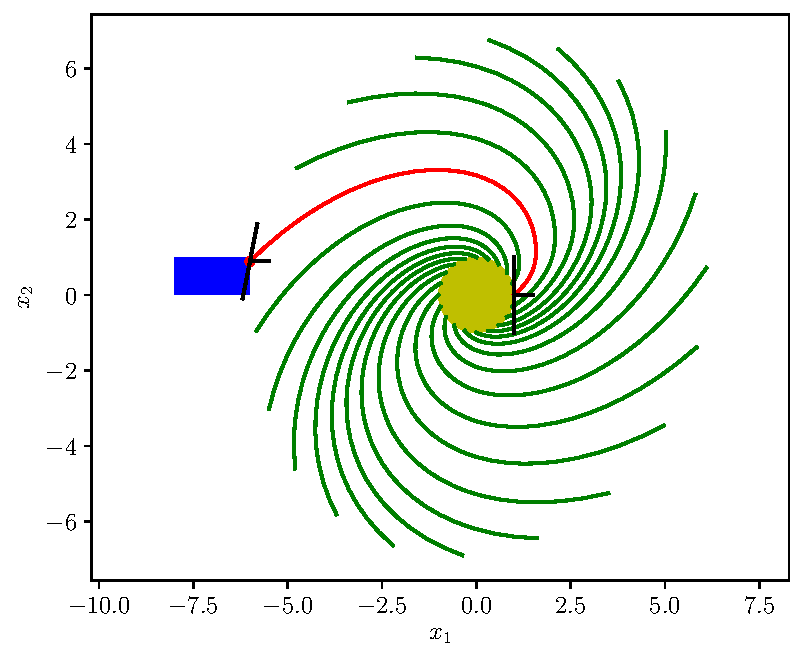
\includegraphics[width=0.9\textwidth]{figures/ex1_x.pdf}
        \label{fig:ex1_x}
        \caption{График примера 1 $(x_2, x_1)$}
    \end{centering}
    \vfill
    \begin{multicols}{2}
        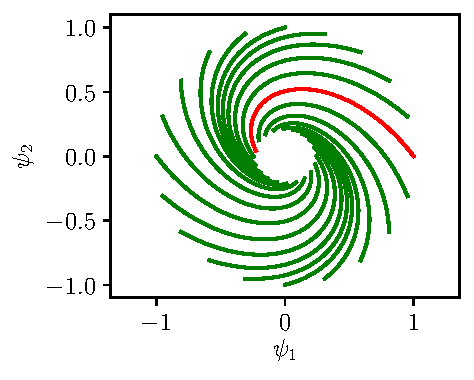
\includegraphics[width=0.5\textwidth]{figures/ex1_p.pdf}
        \label{fig:ex1_p}
        \caption{График примера 1 $(\psi_2, \psi_1)$}
       \hfill 
       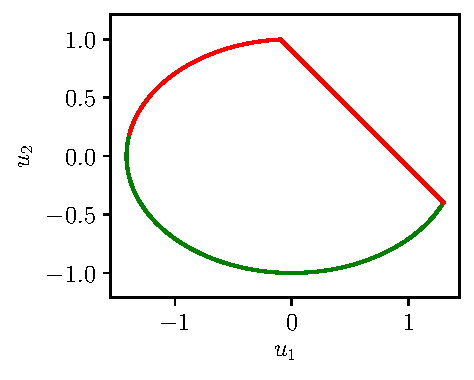
\includegraphics[width=0.5\textwidth]{figures/ex1_u.pdf}
        \label{fig:ex1_u}
        \caption{График примера 1 $(u_2, u_1)$}
    \end{multicols}
\end{figure} 

\begin{figure}[H]
    \begin{multicols}{2}
        \begin{centering}
            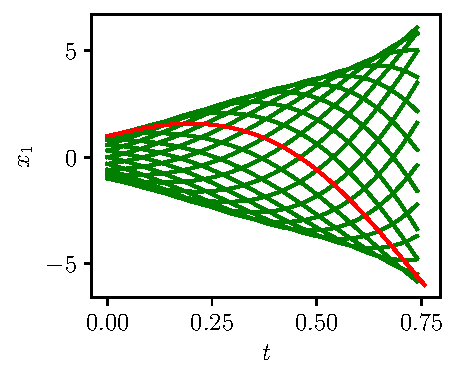
\includegraphics[width=0.48\textwidth]{figures/ex1_x1t.pdf}
            \label{fig:ex1_x1t}
            \caption{График примера 1 $(x_1, t)$}
            \hfill 
            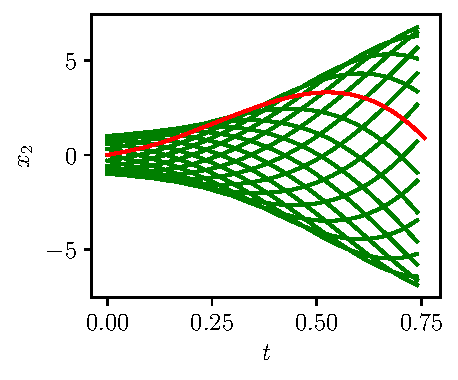
\includegraphics[width=0.48\textwidth]{figures/ex1_x2t.pdf}
            \label{fig:ex1_x2t}
            \caption{График примера 1 $(x_2, t)$}
        \end{centering} 
    \end{multicols}
    \vfill
    \begin{multicols}{2}
        \begin{centering}
            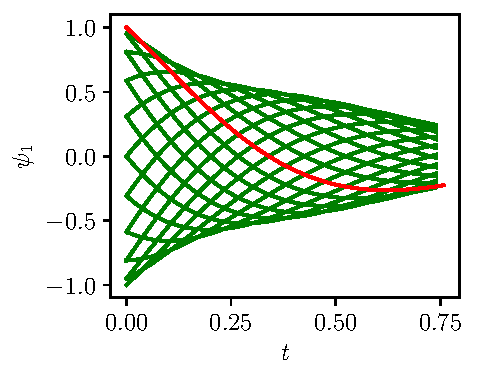
\includegraphics[width=0.48\textwidth]{figures/ex1_p1t.pdf}
            \label{fig:ex1_p1t}
            \caption{График примера 1 $(\psi_1, t)$}
            \hfill 
            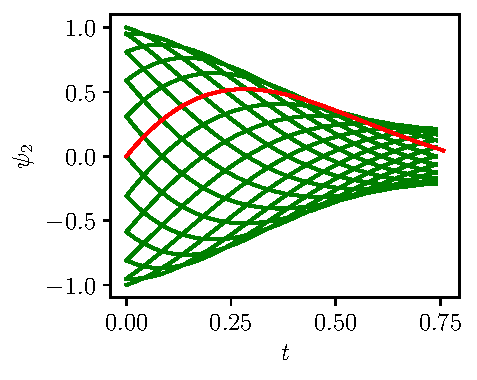
\includegraphics[width=0.48\textwidth]{figures/ex1_p2t.pdf}
            \label{fig:ex1_p2t}
            \caption{График примера 1 $(\psi_2, t)$}
        \end{centering} 
    \end{multicols}
    \vfill
    \begin{multicols}{2}
        \begin{centering}
            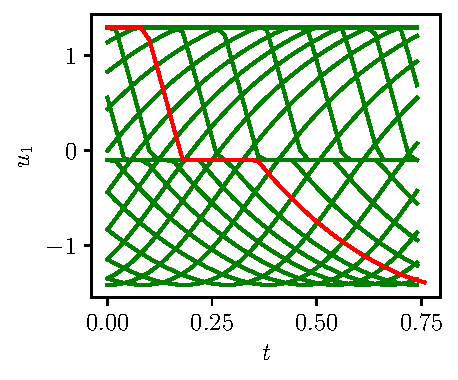
\includegraphics[width=0.48\textwidth]{figures/ex1_u1t.pdf}
            \label{fig:ex1_u1t}
            \caption{График примера 1 $(u_1, t)$}
            \hfill 
            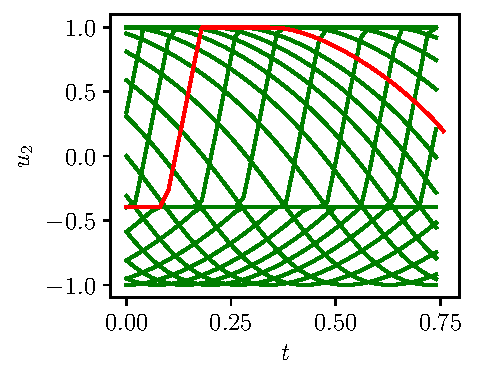
\includegraphics[width=0.48\textwidth]{figures/ex1_u2t.pdf}
            \label{fig:ex1_u2t}
            \caption{График примера 1 $(u_2, t)$}
        \end{centering} 
    \end{multicols}
\end{figure} 

\begin{figure}[H]
    \centering
    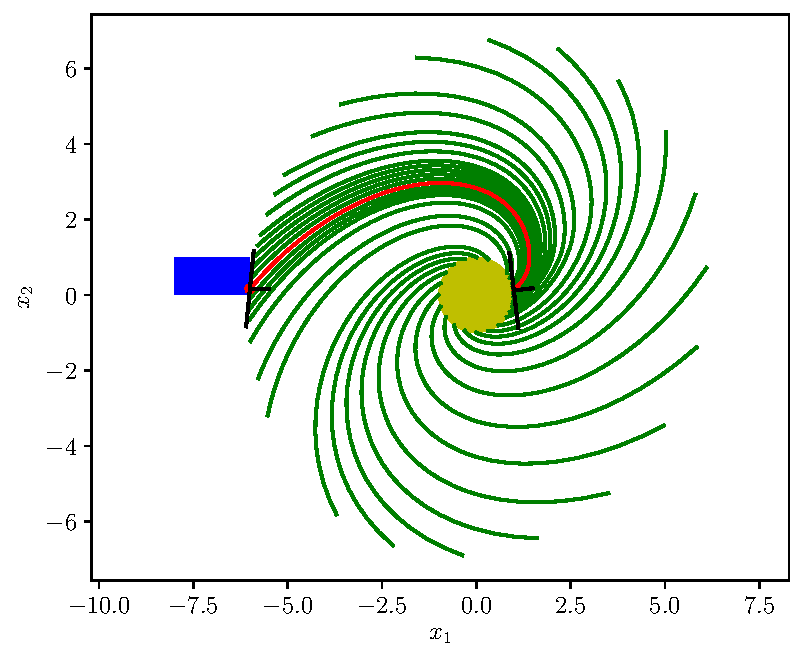
\includegraphics[width=0.9\textwidth]{figures/ex1_x_clar.pdf}
    \label{fig:ex1_clar}
    \caption{Траектории примера 1 после уточнения}
\end{figure} 

\paragraph{Пример 2}

Параметры модели:

\[
    A(t) = 
    \left(\begin{array}{cc}
            e^{-t} & -t^2 \\
            t & \sin t
    \end{array}\right), \quad 
    B(t) = \left(
    \begin{array}{cc}
        1 & 0 \\
        0 & 1
    \end{array} \right), \quad 
    f(t) = \left( 
        \begin{array}{cc}
        \sin t \\ 2\cos t
    \end{array} 
    \right), \quad t_0 = 0,
\]
\[
    \mathcal{X}_0 = B_1(0), \quad
    \mathcal{X}_1 = \conv \left\{ 
        (-10, 0), (-9, 1), (-8, 0), (-7, 1)
    \right\}
,\] 
\[
    \mathcal{P} = \left\{ (x_1, x_2) \in \Real^2 \Bigm| 
    2x_1^2 + x_2^2 \le 1,\
    x_1 + x_2 \le 0.9\right\}
.\] 

Субоптимальное время перехода на 1-й итерации составило $1{,}6903$.
Ошибка условия трансверсальности~---~$0{,}0801$.
После 3-х итераций уточнения сетки субоптимальное время составило 
$1{,}6303$, а ошибка трансверсальности~---~$0{,}0035$.

\begin{figure}[H]
    \begin{centering}
        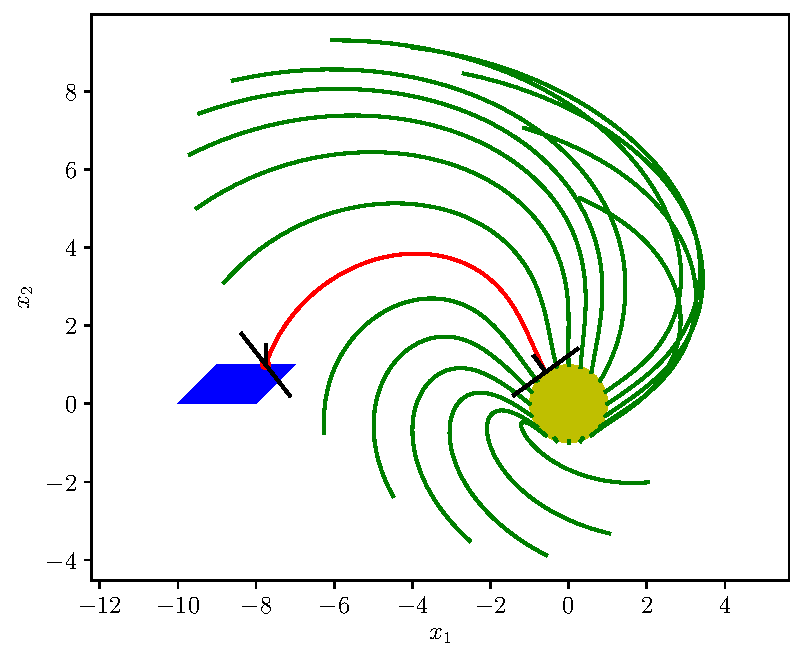
\includegraphics[width=0.9\textwidth]{figures/ex2_x.pdf}
        \label{fig:ex2_x}
        \caption{График примера 2 $(x_2, x_1)$}
    \end{centering}
    \vfill
    \begin{multicols}{2}
        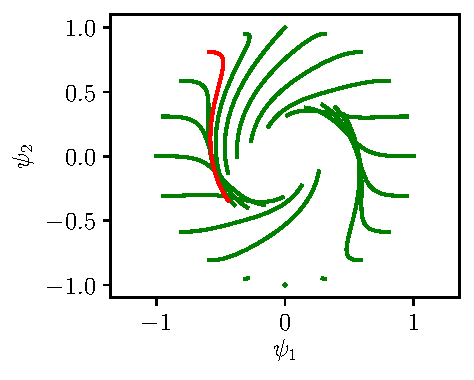
\includegraphics[width=0.5\textwidth]{figures/ex2_p.pdf}
        \label{fig:ex2_p}
        \caption{График примера 2 $(\psi_2, \psi_1)$}
       \hfill 
       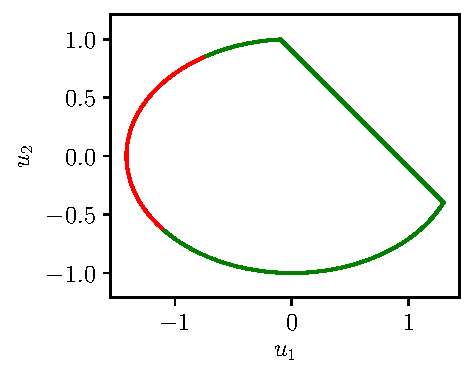
\includegraphics[width=0.5\textwidth]{figures/ex2_u.pdf}
        \label{fig:ex2_u}
        \caption{График примера 2 $(u_2, u_1)$}
    \end{multicols}
\end{figure} 

\begin{figure}[H]
    \begin{multicols}{2}
        \begin{centering}
            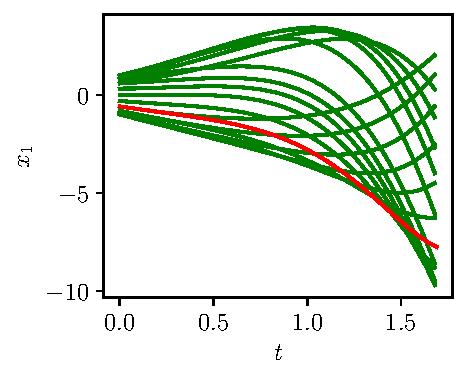
\includegraphics[width=0.48\textwidth]{figures/ex2_x1t.pdf}
            \label{fig:ex2_x1t}
            \caption{График примера 2 $(x_1, t)$}
            \hfill 
            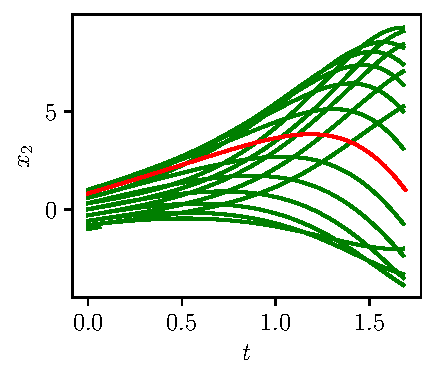
\includegraphics[width=0.48\textwidth]{figures/ex2_x2t.pdf}
            \label{fig:ex2_x2t}
            \caption{График примера 2 $(x_2, t)$}
        \end{centering} 
    \end{multicols}
    \vfill
    \begin{multicols}{2}
        \begin{centering}
            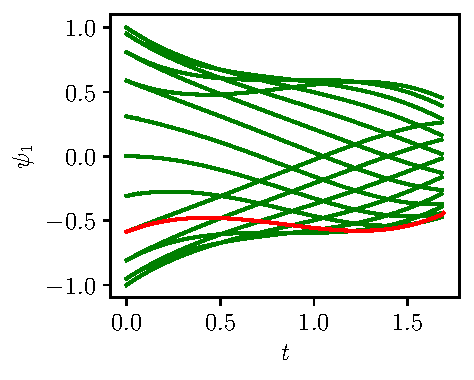
\includegraphics[width=0.48\textwidth]{figures/ex2_p1t.pdf}
            \label{fig:ex2_p1t}
            \caption{График примера 2 $(\psi_1, t)$}
            \hfill 
            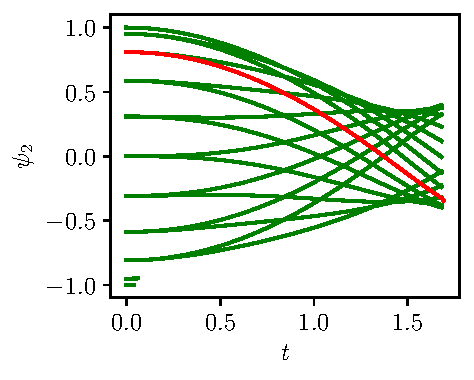
\includegraphics[width=0.48\textwidth]{figures/ex2_p2t.pdf}
            \label{fig:ex2_p2t}
            \caption{График примера 2 $(\psi_2, t)$}
        \end{centering} 
    \end{multicols}
    \vfill
    \begin{multicols}{2}
        \begin{centering}
            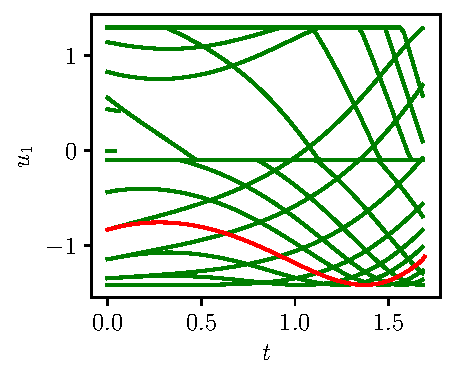
\includegraphics[width=0.48\textwidth]{figures/ex2_u1t.pdf}
            \label{fig:ex2_u1t}
            \caption{График примера 2 $(u_1, t)$}
            \hfill 
            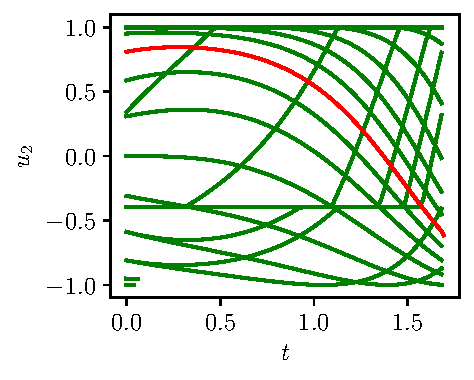
\includegraphics[width=0.48\textwidth]{figures/ex2_u2t.pdf}
            \label{fig:ex2_u2t}
            \caption{График примера 2 $(u_2, t)$}
        \end{centering} 
    \end{multicols}
\end{figure} 

\begin{figure}[H]
    \centering
    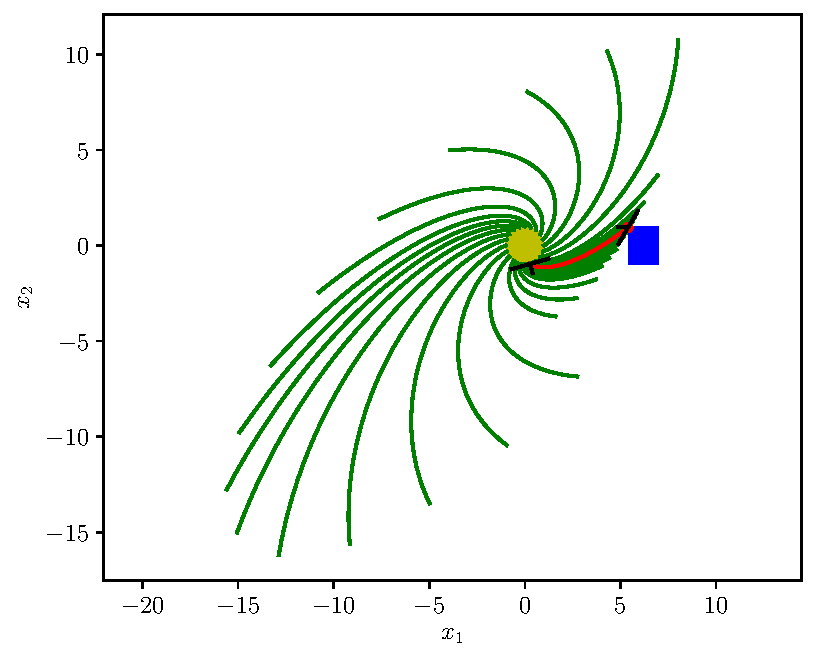
\includegraphics[width=0.9\textwidth]{figures/ex2_x_clar.pdf}
    \label{fig:ex2_clar}
    \caption{Траектории примера 2 после уточнения}
\end{figure} 

\section{Исследование зависимости $t_1^*$ от параметров модели}

В данном разделе исследуется вопрос разрывности оптимального 
времени перехода в зависимости от входных параметров. 

\subsection{Разрыв 1-го рода}

Разрыв 1-го рода можно продемонстрировать на следующей модели:

\[
    A(t) = 
    \left(\begin{array}{cc}
            0 &-2 \\
            2 & 0
    \end{array}\right), \quad 
    B(t) = \left(
    \begin{array}{cc}
        1 & 0 \\
        0 & 1
    \end{array} \right), \quad 
    f(t) = \left( 
        \begin{array}{cc}
        0 \\ 0
    \end{array} 
    \right), \quad t_0 = 0,
\]
\[
    \mathcal{X}_0 = B_{0{,}1}\left( 0\right), \quad
    \mathcal{X}_1 = \conv \left\{ 
        (0; 3{,}7), (0; 5), (1; 3{,}7), (1; 5)
    \right\}
,\] 
\[
    \mathcal{P} = \left\{ (x_1, x_2) \in \Real^2 \Bigm| 
        (x_1 + 2)^2 + x_2^2 \le 1,\
    x_1 + x_2 \le 6\right\}
.\] 

При такой конфигурации время быстродействия составит $1{,}6072$.
Но если нижний отрезок прямоугольника положить на уровень  $3{,}8$ вместо 
$3{,7}$ то при данных ограничениях на управление системе понадобится
совершить уже 2 оборота, чтобы попасть в конечное множество.
Оптимальное время перехода составит уже  $3{,}5575$.

\begin{figure}[H]
    \begin{multicols}{2}
        \begin{centering}
            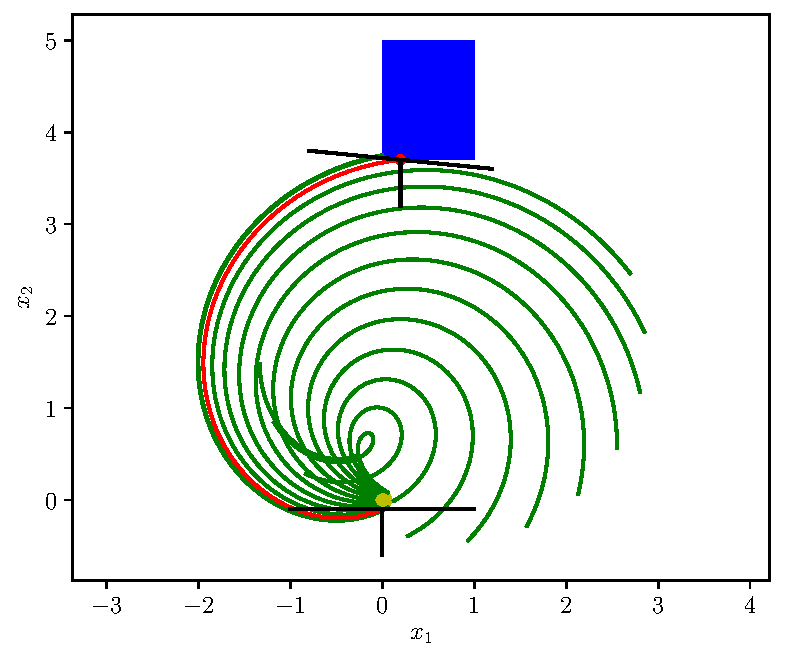
\includegraphics[width=0.48\textwidth]{figures/ex31_x.pdf}
            \label{fig:ex31_x}
            \caption{Нижняя грань квадрата на уровне $3{,}7$. $t_1^{*} = 1{,}6072$}
            \hfill 
            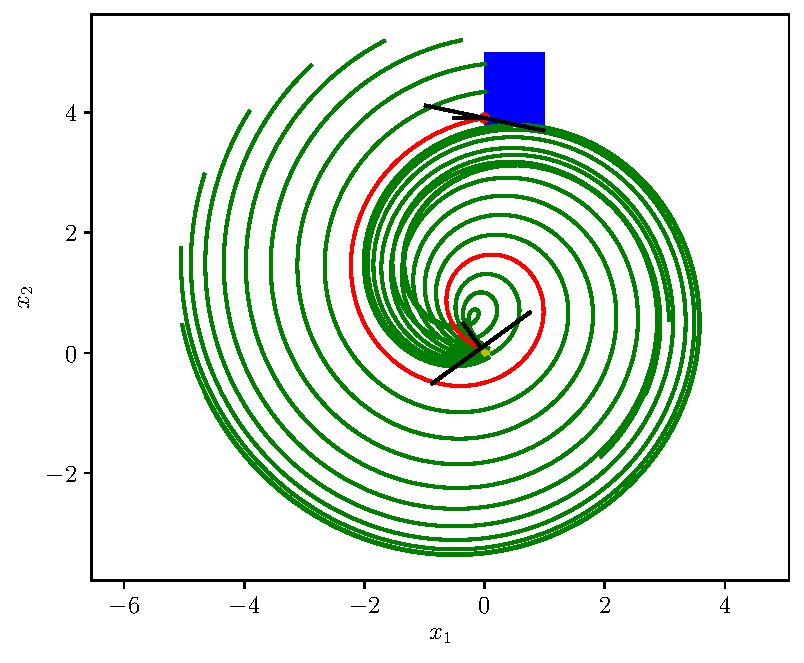
\includegraphics[width=0.48\textwidth]{figures/ex32_x.pdf}
            \label{fig:ex32_x}
            \caption{Нижняя грань квадрата на уровне $3{,}8$. $t_1^{*} = 3{,}5575$}
        \end{centering} 
    \end{multicols}
\end{figure} 

\subsection{Разрыв 2-го рода}


Разрыв 2-го рода можно продемонстрировать на следующей модели:

\[
    A(t) = 
    \left(\begin{array}{cc}
            0 & 0 \\
            0 & 0
    \end{array}\right), \quad 
    B(t) = \left(
    \begin{array}{cc}
        1 & 0 \\
        0 & 1
    \end{array} \right), \quad 
    f(t) = \left( 
        \begin{array}{cc}
        0 \\ 0
    \end{array} 
    \right), \quad t_0 = 0,
\]
\[
    \mathcal{X}_0 = B_{0{,}1}\left( 0\right), \quad
    \mathcal{X}_1 = \conv \left\{ 
        (1{,}4; 1), (1{,}4; -1), (3; 1), (3; -1)
    \right\}
,\] 
\[
    \mathcal{P} = \left\{ (x_1, x_2) \in \Real^2 \Bigm| 
        (x_1 + 1)^2 + x_2^2 \le 1,\
    x_1 + x_2 \le 6\right\}
.\] 

В данном случае пример тривиальный.
Система движется туда, куда ей <<скажет>> управление.
Пользуясь свободой выбора $\mathcal{P}$, рассмотрим 2 случая.
Если управления с положительной первой координатой недопустимы, то 
система не будет <<ехать>> вправо и никогда не достигнет конечного множества.
Но если разрешить такие управления, то будут существовать траектории, 
идущие в положительном направлении оси  $Ox_1$.
Например, положим 

\[
    \mathcal{P} = \left\{ (x_1, x_2) \in \Real^2 \Bigm| 
        (x_1 + 0{,}9)^2 + x_2^2 \le 1,\
    x_1 + x_2 \le 6\right\}
.\] 

\begin{figure}[H]
    \begin{multicols}{2}
        \begin{centering}
            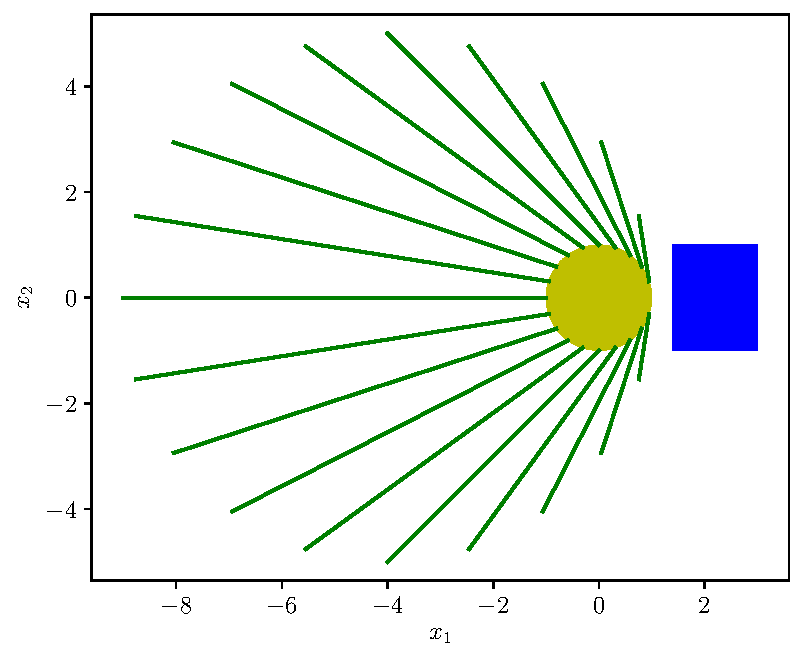
\includegraphics[width=0.48\textwidth]{figures/ex41_x.pdf}
            \label{fig:ex31_x}
            \caption{$\{u_1 > 0\} \notin \mathcal{P}$. $t_1^{*} = \infty$}
            \hfill 
            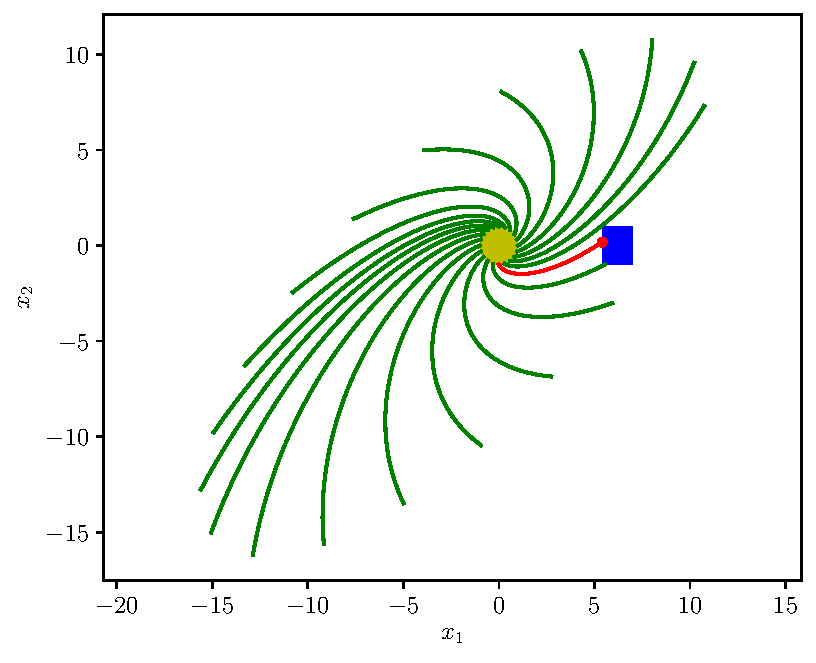
\includegraphics[width=0.48\textwidth]{figures/ex42_x.pdf}
            \label{fig:ex32_x}
            \caption{$\{u_1 > 0\} \in \mathcal{P}$. $t_1^{*} = 4$}
        \end{centering} 
    \end{multicols}
\end{figure} 

\bibliographystyle{utf8gost705u}
\bibliography{biblio}

\end{document} 
